This section examines the equilibrium path of drilling for each of the endogenous and exogenous oil prices. In the endogenous-price scenario, the market clearing oil price is determined from equation (\ref{Equation:Firms-Problem_Oil-Prices}). Moreover, the exogenous price means the case of a constant oil price, in which the oil production industry is small relative to the world oil market.\footnote{In other words, $\widebar{p}_{1} = 0$ in equation (\ref{Equation:Firms-Problem_Oil-Prices}) in the exogenous-price scenario.}
 
\afterpage{
    \begin{figure}[t!]
        \centering
        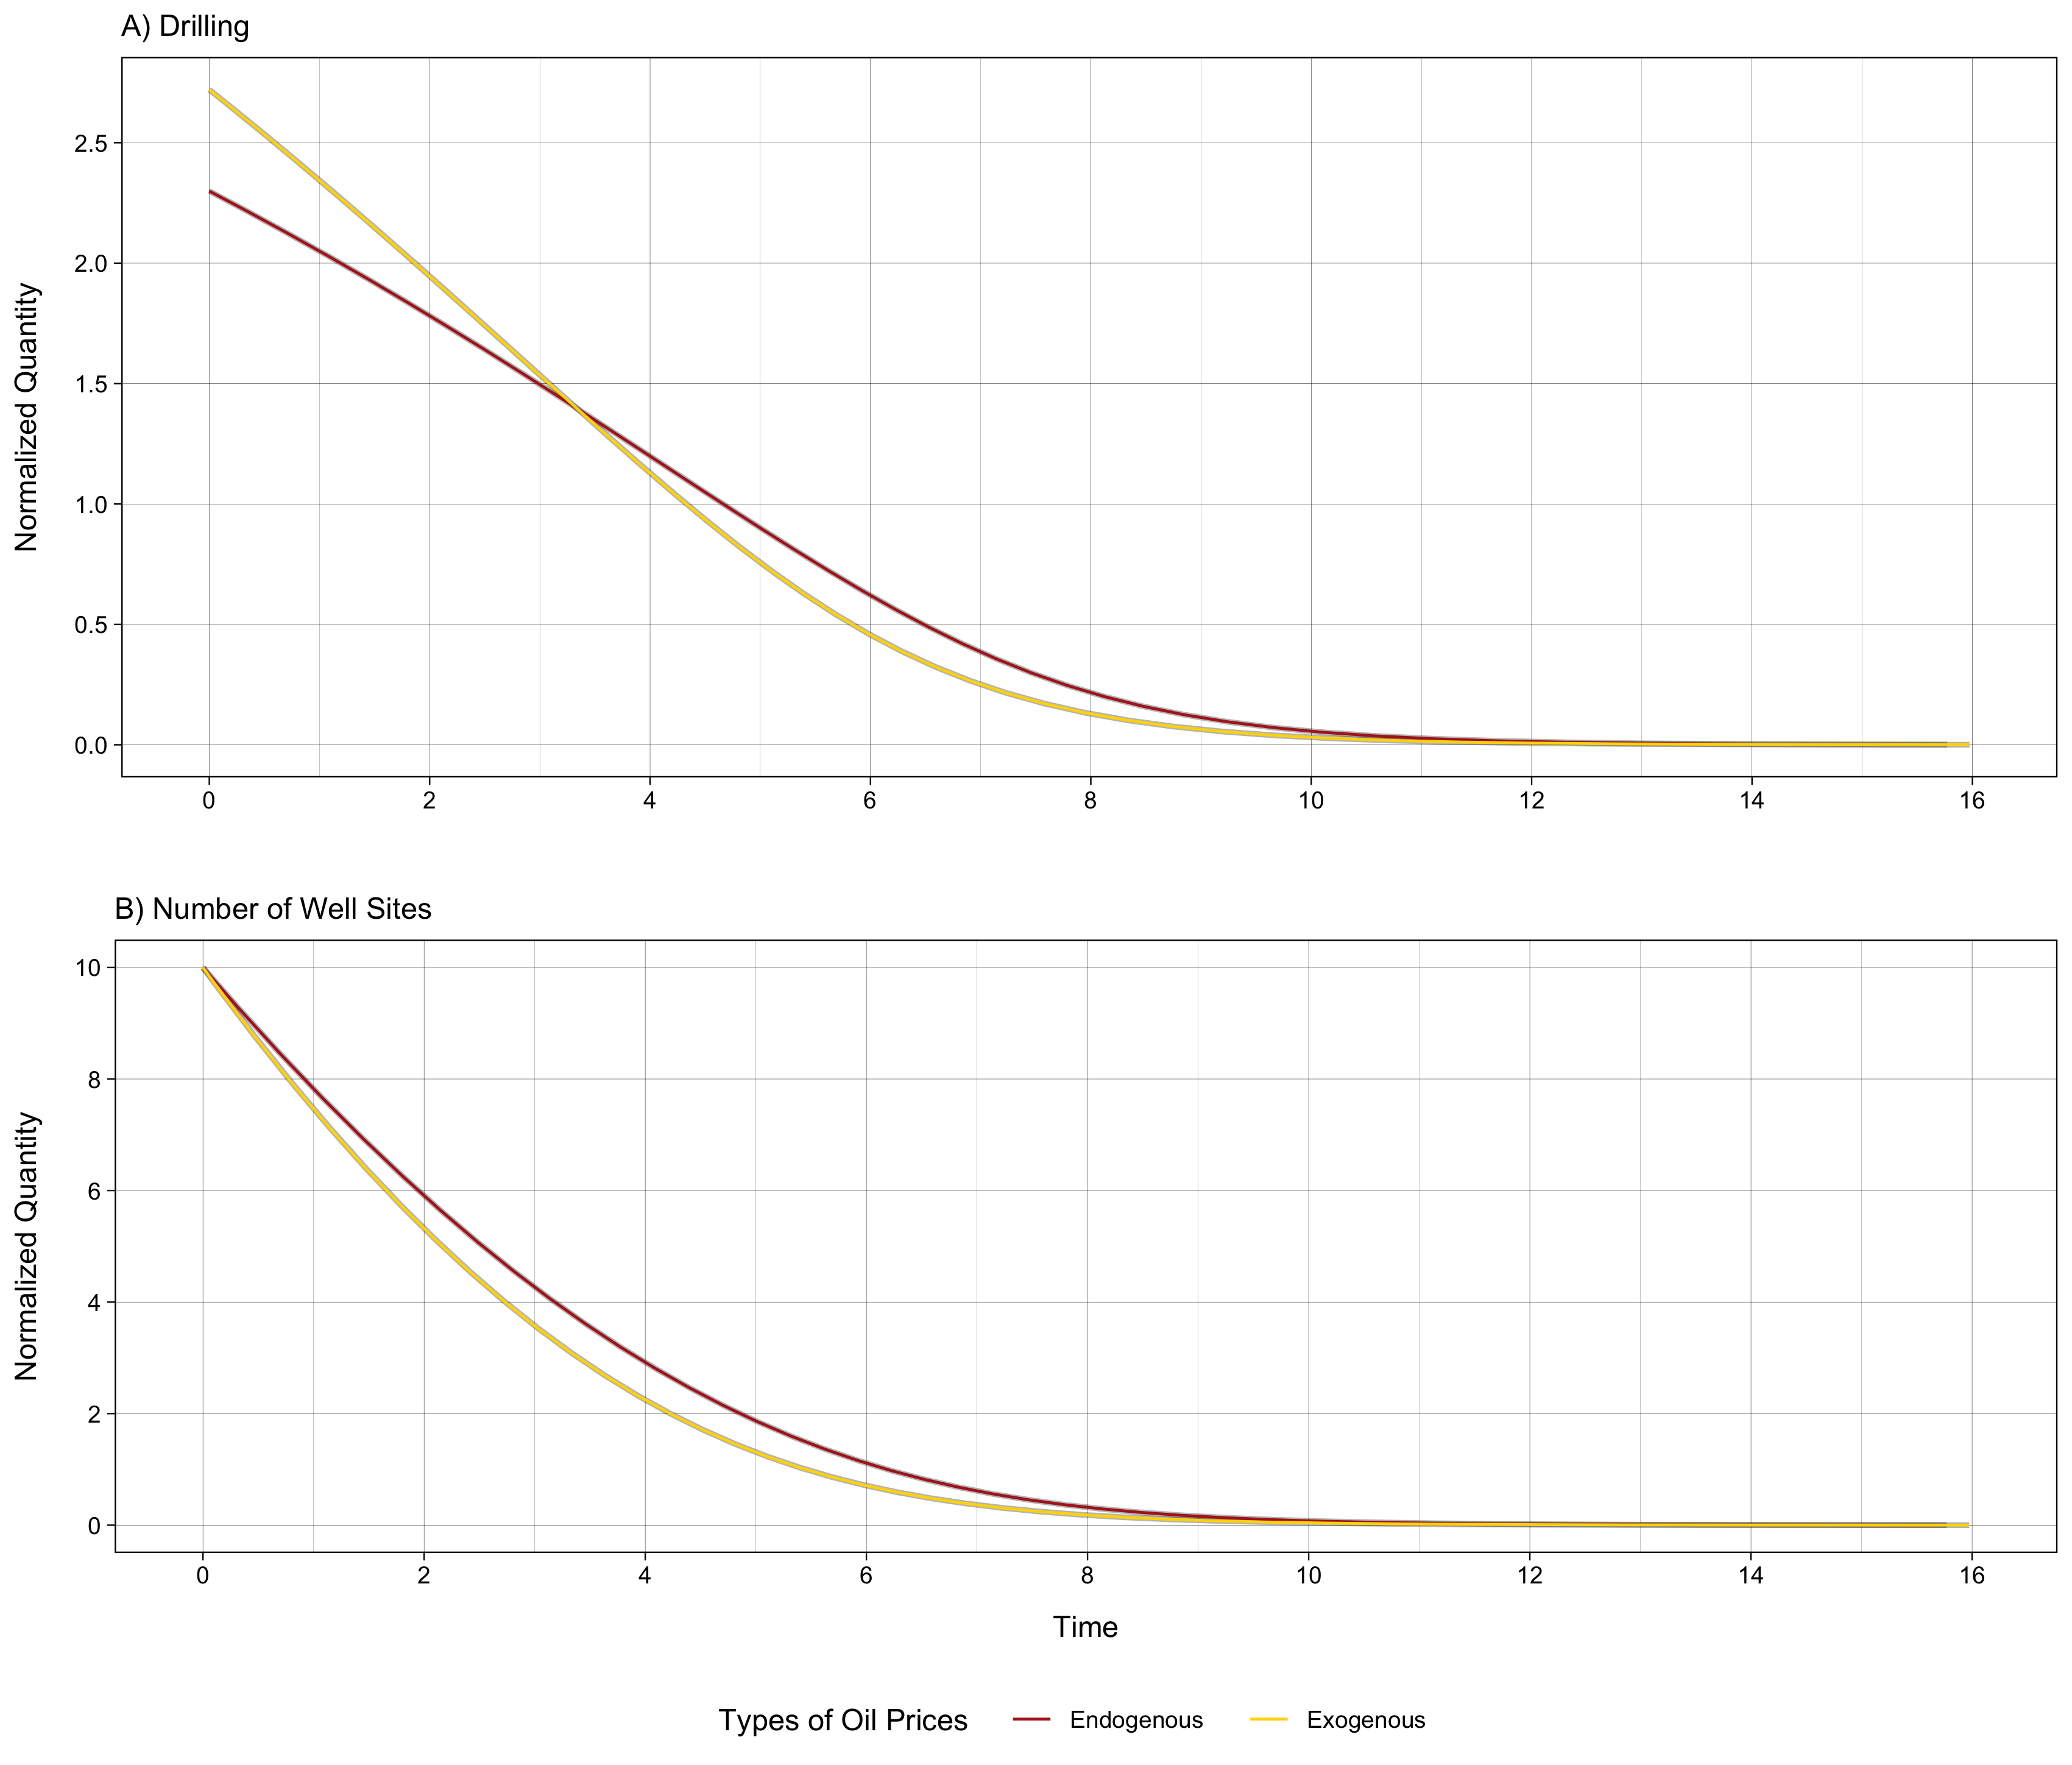
\includegraphics[scale = 0.13]{04_Chapter-3/00A_Figures/Figure_Reserves-and-Drilling-Paths_Endogenous-and-Exogenous-Prices.png}
        \caption{Time Paths under Endogenous and Exogenous Oil Prices}
        \caption*{
            {\small
            \textit{Note}: 
            This figure depicts differences in the time paths for drilling and the measure of well locations under endogenous and exogenous oil prices. This figure takes the assumptions exploited in Figure \ref{Figure:Phase-Diagram_Saddle-Point}. See the text for details.
        }}
        \label{Figure:Time-Paths-for-Drilling-and-Reserves-under-Endogenous-and-Exogenous-Oil-Prices}
    \end{figure}
}
The Euler equation (\ref{Equation:Firms-Problem_Euler-Equation}) allows us to predict the differences in drilling and production time paths between the two price scenarios. The endogenous price is lower than the exogenous price when there is oil production (i.e., $Q > 0$). In the Euler equation, a lower price, thus a lower instantaneous payoff of drilling (i.e., $\psi_{i1k}$),  implies a lower probability of drilling. In other words, endogenizing the time path of oil prices makes the probability of drilling at time $t = 0$ decrease due to the initial production (i.e., $Q_{0} > 0$). Since increasing drilling, and thus production, causes oil prices endogenously determined to fall, there would be no incentive to rapidly raise the rate of drilling. For these reasons, drilling under endogenous oil prices (denoted $D_{t}^{en}$) would be small relative to that under exogenous oil prices (denoted $D_{t}^{ex}$) for some period after $t = 0$. But at some time point, $D_{t}^{en}$ would be larger than $D_{t}^{ex}$ because of the lower level of undrilled reserves in the exogenous-price case. Figure \ref{Figure:Time-Paths-for-Drilling-and-Reserves-under-Endogenous-and-Exogenous-Oil-Prices}, which shows the time paths for drilling and the remaining reserves for each type of oil price, supports the predictions.
